\chapter{Resultados e Discussão}
\label{chap:resultados}

\begin{introduction}
Este capítulo apresenta o estado final da solução, as decisões tomadas durante o desenvolvimento e discute os pontos fortes e fracos do sistema escolhido.
\end{introduction}

\section{Estado Final da Solução e Decisões de Implementação}

Apesar da arquitetura nos permitir ter uma visão geral e antecipar possíveis decisões (como a escolha das tecnologias), o desenvolvimento continua a requerer a tomada de decisões, quer pela escolha de implementações específicas de certas tecnologias, quer pela ocorrência de problemas inesperados.
Por esta razão, apresento a seguir o estado final da solução (Figura~\ref{sys_arq_deployment}) e as escolhas tomadas durante o desenvolvimento.

\begin{figure}[h]
    \centering
    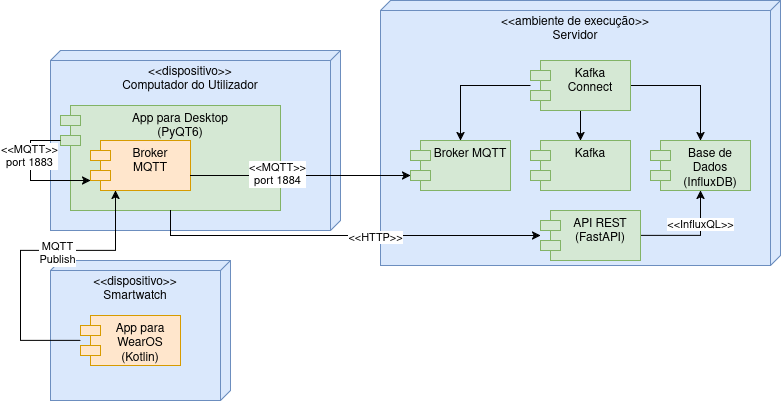
\includegraphics[width=\linewidth]{figs/deployment_arquitecture.png}
    \caption{Diagrama de \textit{deployment} do sistema}
    \label{fig:sys_arq_deployment}
\end{figure}

\subsection{Instanciação Tecnológica da \textit{Pipeline} de Ingestão de Dados}

Apesar da escolha mais importante ser no tipo de tecnologia (como \ac{MQTT} ou \ac{TSDB}), o desenvolvimento de uma solução real requer que escolhamos as ferramentas específicas que implementem estas tecnologias.

Para os \textit{brokers} local e remoto, escolhi optar pelo Mosquitto.
Apesar de existirem outras implementações de \ac{MQTT} como o ActiveMQ que possuem melhor \textit{performance} em escala (por utilizarem todos os recursos disponíveis), o Mosquitto continua a ter uma melhor \textit{performance} em cenários com recursos limitados~\cite{Mishra2021}.
Esta qualidade pode ser útil para o \textit{broker} remoto em cenários N:1 (como o descrito na Secção~\ref{sec:chosen_technologies}), mas torna-se particularmente útil para o \textit{broker} local quando este é executado em computadores com recursos mais limitados (como, por exemplo, \textit{Chromebooks}), onde a execução em paralelo com \textit{software} de videochamada (como o Zoom) poderá limitar severamente os recursos disponíveis.
Outra vantagem inerente ao Mosquitto que levou a esta decisão, foi o mecanismo de redirecionamento \textit{\ac{MQTT} Bridge} que permite enviar as mensagens do \textit{broker} local para o \textit{broker} remoto de forma automática sem comprometer as garantias de entrega.

Em termos de armazenamento de dados, decidi optar pelo InfluxDB por ser uma base de dados criada de raiz para lidar com séries temporais, ao contrário de bases de dados como o TimescaleDB, que foi criada como extensão ao PostgreSQL~\cite{influxdata2026}.
Esta diferença permite ao InfluxDB oferecer maior velocidade de ingestão, o que é uma qualidade útil neste caso de uso, que consiste maioritariamente de escritas constantes de pequeno tamanho~\cite{OctaByte2025}.
Finalmente, após a versão 3, o InfluxDB oferece agora a possibilidade de realizar \textit{queries} utilizando \ac{SQL} \textit{standard}~\cite{influxdata2026}, removendo assim a barreira de aprendizagem para programadores, uma das vantagens atribuídas ao TimescaleDB




\section{Fluxo \textit{end-to-end}}

\footnotetext{O MQTT5 Explorer apenas apresenta a última mensagem recebida por tópico, não o histórico completo de mensagens.}




\section{Validação Analítica de Desempenho}

Para além de garantir que a arquitetura do sistema cumpre com os objetivos propostos, é necessário também garantir que as ferramentas utilizadas (principalmente do servidor) são capazes de lidar com o número esperado de mensagens e clientes.

\subsection{Tamanho das Mensagens}

A estrutura da mensagem, serializada em formato \ac{JSON} (como visto na Listagem~\ref{code:example_message}), foi desenhada para ser concisa, apresentando um payload médio de 133B para o \ac{JSON} em si (valor obtido através da serialização de uma das mensagens) e cerca de 173B se incluirmos os \textit{headers} de TCP/IP.

Considerando este volume de dados inexpressivo, o fator determinante para a escalabilidade da infraestrutura é exclusivamente o número de mensagens simultâneas que o broker consegue processar por segundo, e não o tamanho individual de cada pacote. Uma vez que a estrutura é simples e não exige processamento complexo ao nível da camada de transporte, o sistema é capaz de suportar um débito elevado de eventos, sendo a capacidade de ingestão limitada primariamente pela cadência de publicação (\textit{throughput}) e não pela ocupação da largura de banda.

\subsection{Volume de Mensagens Esperado}

O volume de mensagens pode variar com base no número e tipo de sensores, contudo, com base no exemplo atual com 3 sensores, temos o seguinte volume de mensagens:
    
\begin{table}[h]
\centering
\begin{threeparttable}
\caption{Estimativa da frequência de ingestão por dispositivo.}
\label{tab:sensor_throughput}
\begin{tabular}{llc}
\toprule
\textbf{Sensor} & \textbf{Descrição} & \textbf{Frequência (msg/s)} \\ 
\midrule
Teclado\tnote{1} & Eventos de digitação & $5$ \\
WearOS (\ac{BPM})\tnote{2} & Monitorização cardíaca & $1$ \\
Webcam\tnote{3} & Processamento de vídeo/metadados & $10$ \\ 
\midrule
\textbf{Total} & & \textbf{$16$ msg/s} \\ 
\bottomrule
\end{tabular}
\begin{tablenotes}
    \small
    \item[1] Baseado numa taxa de digitação de 60 palavras por minuto (aproximadamente 5 caracteres por segundo).
    \item[2] Frequência nominal de atualização. O sistema opera de forma reativa, pelo que a taxa real de mensagens é dinâmica e proporcional à variação dos valores de \ac{BPM} reportados pelo sensor, não excedendo o limite de $1$ Hz.
    \item[3] A taxa de 10 mensagens por segundo não constitui um limite de hardware, sendo uma configuração definida para satisfazer os requisitos de amostragem necessários para a presente análise.
\end{tablenotes}
\end{threeparttable}
\end{table}

Devido à reduzida carga operacional, o sistema apresenta baixos requisitos computacionais, sendo capaz de operar estavelmente em praticamente qualquer servidor moderno ou computador pessoal, sem necessidade de hardware especializado.
Em termos de número de utilizadores simultâneos, apesar de alguns estudos involverem centenas de voluntários, a necessidade de monitorizar os voluntários tende a limitar este número para um máximo de cerca de 50 utilizadores em simultâneo. Com base neste valor, podemos estimar que a carga máxima esperada para o servidor não irá superar as 800 mensagens por segundo (o que equivale a cerca de 138.4KB/s). 